\documentclass{article}
\usepackage{fullpage}
\usepackage{color}
\usepackage[normalem]{ulem}
\usepackage{hyperref}
\usepackage{enumitem}
\hypersetup{colorlinks}
\usepackage{graphicx}
\hyphenpenalty=100000
\begin{document}
\setlength{\voffset}{3.5in}
\title{Project Plan}
\author{\Large Android Based Situational Awareness: Moving Map\\
Tom Atnip, Susi Cisneros, Sam Kim, and Seth Troisi}
\date{\today}
\maketitle
\clearpage
\setlength{\voffset}{0pt}
\tableofcontents
\clearpage
~\\
\begin{Large}\textbf{Changes}\end{Large}\\
~\\
\begin{tabular}{ | p{1.5in} | p{4.5in} | }
\hline
\textbf{Date} & \textbf{Description}\\
\hline
\hline
September 13, 2012 & Document started\\
\hline
September 20, 2012 & Created outline\\
\hline
September 20, 2012 & Wrote Users/Stakeholders section\\
\hline
September 23, 2012 & Wrote Key Needs, Alternatives, Risks, Documentation Metrics, and Code Metrics\\
\hline
September 24, 2012 & Updated Requirements as per Gate 5 visit with Raytheon\\
\hline
October 4, 2012 & Separate document created\\
\hline
October 8, 2012 & Added fall quarter schedule, added Assumptions and Opportunities, and updated Risks\\
\hline
October 15, 2012 & Added Introduction\\
\hline
\end{tabular}
\clearpage

\section{Introduction}
This document will outline the software process we will use to develop
the system. It will then show the projected schedule, along with any risks.


\section{Description of Processes}
\section{Configuration Management Plan}
For this project we will be using GitHub to share code and documentation with our client. This web service uses git as the versioning control system. The project is an android based mobile application that will be written in Java using the android libraries.  We will be using Eclipse as the development IDE.\\

\section{Schedule}
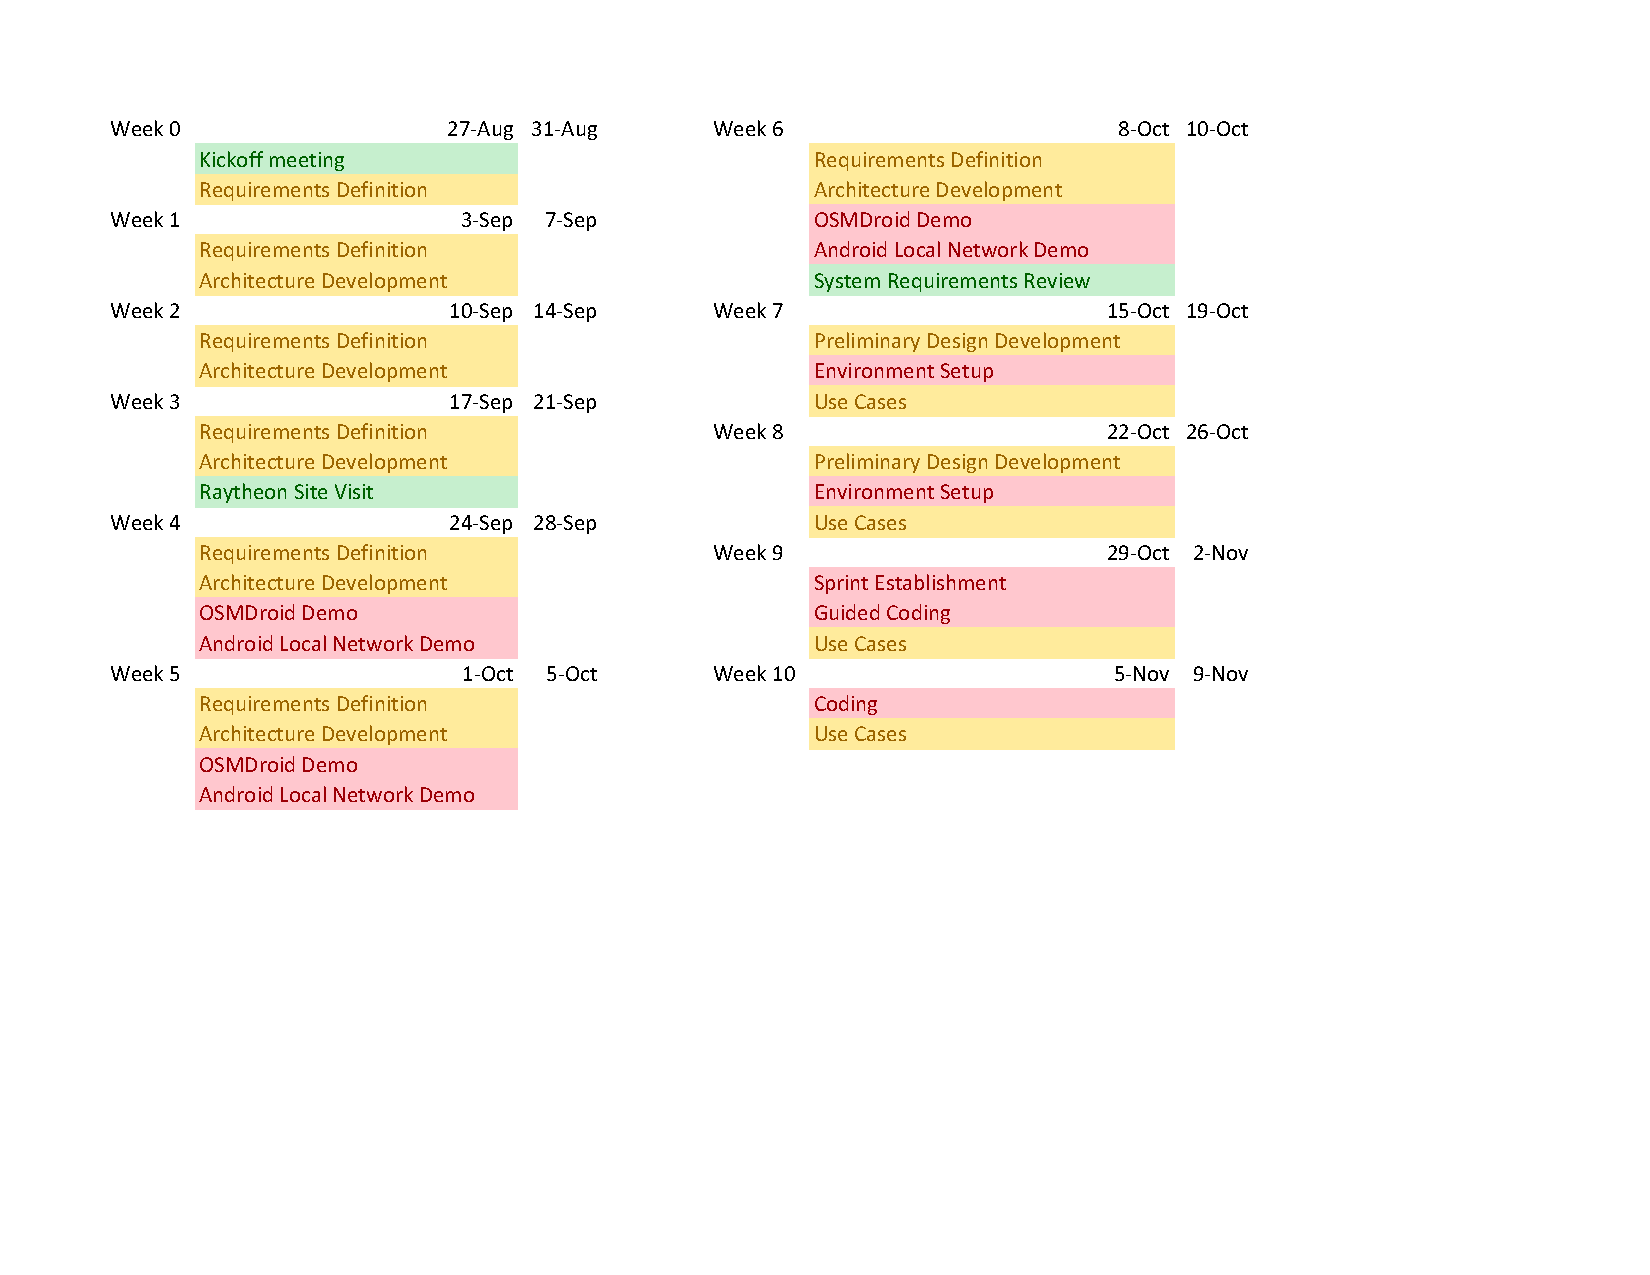
\includegraphics[keepaspectratio, width=8in]{FallSchedule.pdf} \\

\subsection{Assumptions}
\begin{tabular}{ | p{.5in} | p{4.5in} | }
\hline
\textbf{ID} & \textbf{Assumption}\\
\hline
\hline
A0 & There exists an open source mapping engine for Android devices\\
\hline
A1 & The mapping engine does not require an internet connection to run\\
\hline
A2 & Android devices can connect to a local server\\
\hline
\end{tabular}

\subsection{Risks}
\begin{tabular}{ | p{.5in} | p{4.5in} | }
\hline
\textbf{ID} & \textbf{Risk}\\
\hline
\hline
R0 & Performance of the system\\
\hline
R1 & Organizing data in the correct format in a timely manner\\
\hline
\end{tabular}

\subsection{Opportunities}
\begin{tabular}{ | p{.5in} | p{4.5in} | }
\hline
\textbf{ID} & \textbf{Opportunity}\\
\hline
\hline
O0 & Finding a feature complete mapping engine\\
\hline
\end{tabular}


\end{document}